% Generated by segmentation_extension/make_extension.py; do not edit numbers.
\section{Prospective segmentation extension}
\label{app:segmentation}
This extension was preregistered after the historical GPU observations had been inspected; it does not retroactively preregister them. It asks whether instance-mask construction, rather than NMS, supplies a larger per-object cost. Device measurements and attack counts use the first 20 lexicographically ordered images of COCO128-seg, not an independent held-out cohort. The pretrained weights and all image identities are bound by SHA-256 manifests. Digital full-image perturbations are used; physical patches are not evaluated here.
\subsection{Synthetic mask workload and measurement quality}
YOLOv8n-seg is evaluated in FP32 at $640\times640$, confidence 0.25 and IoU 0.45. NMS uses a fixed torchvision kernel. Real image forward and NMS are followed by deterministic injected mask coefficients and boxes at $K\in\{0,10,50,100,300\}$. Total time is measured directly; mask time is also measured separately. The proto-resolution option uses \texttt{upsample=False}, as in the historical microbenchmark, and is not presented as the default deployed predictor. Full-resolution masks use \texttt{process\_mask\_native}.
Each image has five repetitions, randomized condition order, two $K=0$ A/A copies, and a fixed-image forward reference before each image. GPU timers synchronize on both boundaries. CPU affinity is read back and verified under load. The rented host reports an i7-12700K name but exposes 18 homogeneous logical processors; P/E-core or physical-core identities cannot be inferred. The CPU condition below pins logical processors 2--5 with four intra-op threads.
The ratio uses $K=10$ as baseline, per-image medians followed by a geometric mean; confidence intervals resample images 20,000 times with seed 20261106. The MDE is an 80\%-power central-$t$ approximation on the log A/A ratio. $K^*$ is the smallest tested $K>10$ whose lower ratio confidence limit exceeds $\exp(\mathrm{MDE}_{\log})$.
\begin{table*}[t]\centering
\caption{Prospective synthetic mask workload. Ratios are directly measured total time at $K=300$ relative to $K=10$, conditional on the fixed cohort. Only runs meeting the registered quality gate are included.}
\label{tab:seg-device}
\begin{tabular}{llrrrr}\toprule
Device & Mask construction & Total ratio [95\% CI] & MDE (\%) & $K^*$ & Drift flags\\\midrule
CPU, four exposed logical processors & Proto resolution & 1.091 [1.076, 1.107] & 2.07 & 300 & 0 \\
CPU, four exposed logical processors & Full resolution & 3.951 [3.914, 3.996] & 1.61 & 50 & 0 \\
RTX 5060 Ti & Proto resolution & 1.046 [1.032, 1.060] & 1.38 & 300 & 2 \\
RTX 5060 Ti & Full resolution & 1.926 [1.919, 1.934] & 1.88 & 50 & 2 \\
\bottomrule\end{tabular}\end{table*}
\begin{figure*}[t]\centering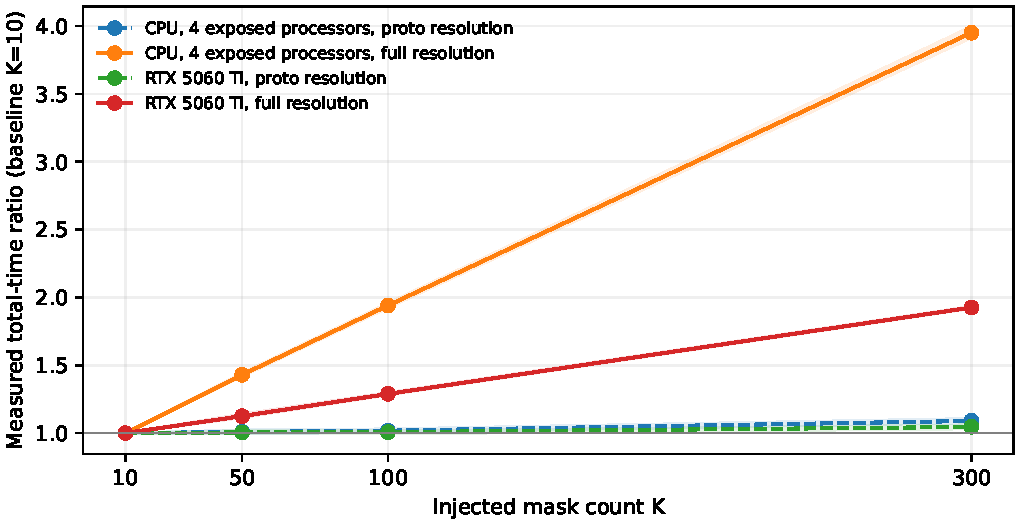
\includegraphics[width=0.85\textwidth]{segmentation_extension/mask_dose_response.pdf}\caption{Synthetic mask-workload dose response on the two quality-accepted device runs. Shading shows image-bootstrap 95\% intervals; the ratio is relative to $K=10$.}\label{fig:seg-dose}\end{figure*}
The CPU-four-processor run has zero flagged reference points and both load checks pass; the GPU run has two flagged points, within the allowed maximum of two. A separate single-processor CPU run has ten flagged points and is excluded from this table. Earlier laptop runs remain rejected. These synthetic controls establish a cost surface, not attack efficacy.
\subsection{Real perturbations and native NMS-free transfer}
The prospective attack confirmation reuses the historical full-image PGD objective and fixed budget ($L_\infty=16/255$, 100 steps, step size $2/255$). It evaluates the final iterate, rather than the best iterate over a trajectory. On YOLOv8n-seg, median retained count changes from 2.5 to 270; 20/20 images reach $K\ge100$ and 6/20 reach the cap of 300.
The SAME perturbations are transferred to YOLO26n-seg with its one-to-one head explicitly enabled ($\texttt{end2end=True}$). Counts come directly from confidence column 4 of the native $[1,300,38]$ output at threshold 0.25, without applying NMS. The target median changes from 2 to 3; 0/20 images reach $K\ge50$. Thus this experiment does not reproduce high-count transfer to the native NMS-free path. It does not establish immunity to a target-specific attack. Earlier high-count YOLO26 observations used a different inference/counting path and cannot support a native NMS-free claim.
\subsection{Expansion to a disjoint 500-image validation cohort}
After the COCO128 observations, a separate prospective study locks 500 of the 5,000 official COCO val2017 images by uniform sampling without replacement (seed 20261106). These images are disjoint from the earlier 20-image cohort. The budget and final-iterate rule are unchanged; FP32 evaluation uses a prospectively fixed batch size of four. Batched kernels can differ numerically from batch-one execution. Each source model optimizes its own perturbations; the YOLO26 target receives the same perturbations optimized on YOLOv8n. Cohorts are reported separately and are not pooled.
\begin{table*}[t]\centering\caption{New COCO-val500 count study. Intervals for medians resample images 20,000 times; proportion intervals use Wilson 95\% bounds. The shared cutoff $K=50$ is a count endpoint, not a calibrated latency threshold for every model.}\label{tab:seg-val500}
\begin{tabular}{lrrlr}\toprule Model/path & Images & Clean median $K$ & Attacked median $K$ [95\% CI] & $K\ge50$ count [95\% fraction CI]\\\midrule
YOLOv8n-seg & 500 & 4 & 300 [300, 300] & 500/500 [99.24\%, 100.00\%] \\
YOLO11n-seg & 500 & 3 & 300 [300, 300] & 500/500 [99.24\%, 100.00\%] \\
YOLO26 native, transfer & 500 & 3 & 3 [3, 4] & 0/500 [0.00\%, 0.76\%] \\
\bottomrule\end{tabular}\end{table*}
\begin{figure*}[t]\centering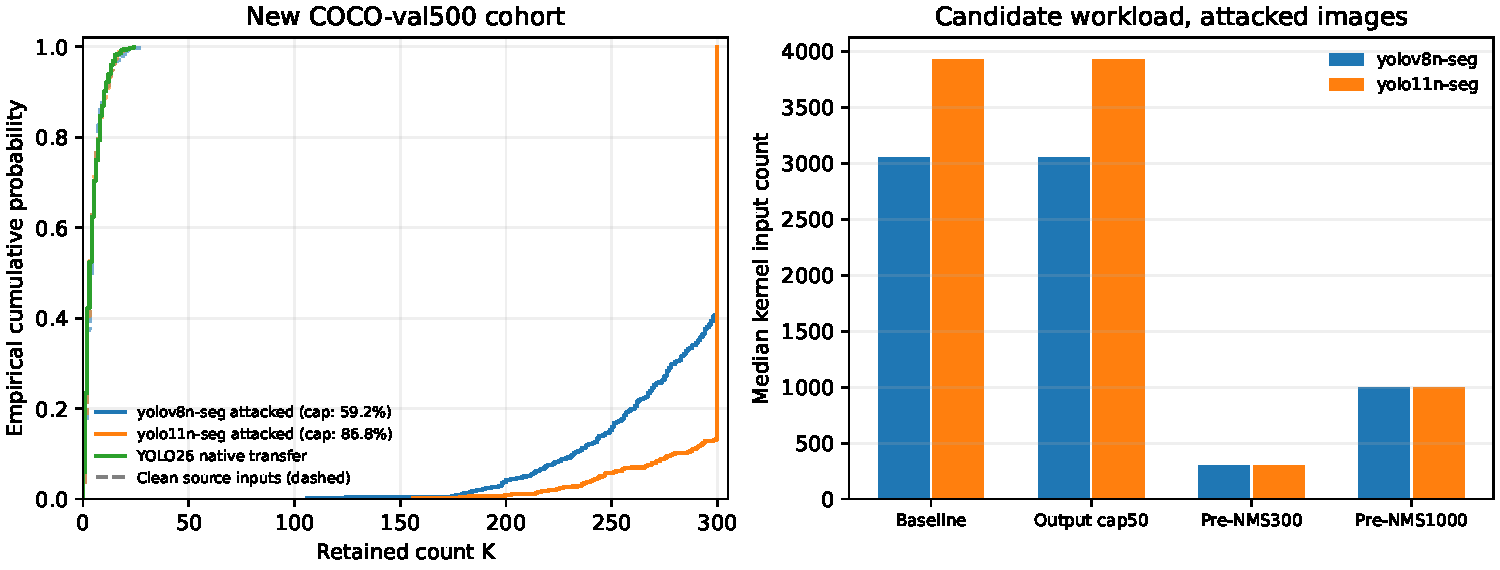
\includegraphics[width=0.95\textwidth]{segmentation_extension/val500_counts.pdf}\caption{Disjoint COCO-val500 cohort. Left: empirical count distributions; dashed curves are clean source inputs, solid curves are attacked source inputs or native transfer. The terminal mass at $K=300$ is the output cap. Right: median candidate counts reaching the fixed NMS kernel. Workload counts do not by themselves establish latency reduction or denial of service.}\label{fig:seg-val500}\end{figure*}
The expanded study includes all outcomes at four cap settings and preserves float32 perturbation arrays, native outputs and hashes. Attack/count inputs use direct square resizing, whereas the separate clean-accuracy validation uses letterboxing; these do not define a jointly matched accuracy--latency curve. Source-model comparisons are descriptive, not causal attribution to architecture. Reaching a count cutoff can include images already above the cutoff when clean; paired gains and newly crossing images are reported in the evidence report. This count study does not convert rejected timing sessions into valid latency evidence and does not establish target-specific robustness of YOLO26.
\subsection{Backend identity and real-pipeline timing}
Inspection of the installed Ultralytics source identifies import-dependent dispatch: when torchvision is present in \texttt{sys.modules}, the wrapper calls \texttt{torchvision.ops.nms}; otherwise it calls \texttt{TorchNMS.nms}. The original scripts differed in this import. A same-tensor kernel comparison reproduced the discrepancy, but that full diagnostic failed its reference-drift gate and is retained as diagnostic evidence rather than a clean headline latency estimate. A separately registered fixed-kernel real-pipeline confirmation is reported in the accompanying evidence package. This source-level distinction precludes attributing the historical large slowdown to mask construction alone.
\subsection{Clean-data accuracy of output and candidate caps}
All 5,000 COCO val2017 images are evaluated using Ultralytics polygon-label segmentation metrics, not an independently recomputed official COCO API score. Inference uses $640$-px letterboxing, FP32, batch size 8, confidence 0.001, IoU 0.7 and workers 0. The lower confidence threshold is the fixed accuracy-evaluation setting, distinct from the attack threshold. Detection-level metric inputs are retained for replay.
\begin{table}[t]\centering
\caption{Full validation segmentation mAP50--95 and absolute change in percentage points.}
\label{tab:seg-defense}
\begin{tabular}{llrr}\toprule Model & Setting & mAP (\%) & $\Delta$ (pp)\\\midrule
yolov8n-seg & Baseline & 30.23 & +0.00 \\
yolov8n-seg & Output cap 50 & 29.85 & -0.38 \\
yolov8n-seg & Pre-NMS cap 300 & 30.01 & -0.22 \\
yolov8n-seg & Pre-NMS cap 1000 & 30.22 & -0.01 \\
yolo11n-seg & Baseline & 31.88 & +0.00 \\
yolo11n-seg & Output cap 50 & 31.48 & -0.40 \\
yolo11n-seg & Pre-NMS cap 300 & 31.64 & -0.25 \\
yolo11n-seg & Pre-NMS cap 1000 & 31.88 & +0.00 \\
\bottomrule\end{tabular}\end{table}
An output cap limits the number of masks but does not bound work before NMS. A pre-NMS cap limits candidate workload and has a separate accuracy cost. These clean-data results alone do not establish attack resistance or statistical equivalence. No significance claim is inferred from small descriptive mAP differences.
A separately registered count-only replay on the 20 frozen attacked inputs confirms the boundary distinction: an output cap of 50 leaves the kernel input count unchanged (1728--3744), whereas the pre-NMS cap of 300 restricts the kernel to 300 candidates on every image. The retained-count median after that pre-NMS cap is 98; this does not establish elimination of mask cost or a measured latency benefit.
\paragraph{Reproducibility and limits.} The device and native-count runs are registered under \texttt{prereg-m2-m3-confirmation-20261106}, with an explicit native-head amendment before count observations. Accuracy evaluation is registered under \texttt{prereg-coco-defense-20261106}; implementation-only amendments and failed smoke runs are retained. The generated source map lists every table input. The study covers one rented host/GPU, fixed small timing/attack cohorts, synthetic mask-workload controls, and digital full-image attacks. It does not establish camera or edge-device denial of service.
\subsection{Nested cohorts and target-specific attacks on an NMS-free model}
\label{sec:nested1500}
We recomputed a nested 1,000/1,500-image COCO-val cohort with five starts per image and four attack paths (30,000 image--start attacks). The prefixes are not independent replications. All paths use 100 PGD steps, $\epsilon=16/255$, $\alpha=2/255$, FP32 unfused evaluation, and the final iterate. A zero start and four image-keyed uniform random starts were fixed prospectively. The two target-specific objectives share the same initial perturbation for each image and start.
\begin{table*}[t]\centering\small
\caption{Nested cohort count endpoints. K is averaged over five starts per image before taking the median. Reach is the average image--start fraction; hierarchical 95\% intervals resample images then starts within each sampled image (20,000 draws). Native outputs use score column 4 above 0.25 and no NMS.}
\label{tab:nested1500}\begin{tabular}{rlrr}\hline
Images & Objective/evaluation & Median K [95\% CI] & Reach $K\geq50$ (\%)\\\hline
1000 & v8/own & 289.40 [288.60, 292.20] & 100.00 [100.00, 100.00]\\
1000 & 11/own & 300.00 [300.00, 300.00] & 100.00 [100.00, 100.00]\\
1000 & v8/native26 & 3.00 [2.80, 3.40] & 0.00 [0.00, 0.00]\\
1000 & 11/native26 & 2.80 [2.60, 3.00] & 0.00 [0.00, 0.00]\\
1000 & 26-many/native26 & 287.60 [287.60, 291.90] & 99.98 [99.92, 100.00]\\
1000 & 26-native/native26 & 217.80 [215.30, 221.20] & 99.92 [99.78, 100.00]\\
1500 & v8/own & 289.40 [289.30, 292.20] & 100.00 [100.00, 100.00]\\
1500 & 11/own & 300.00 [300.00, 300.00] & 100.00 [100.00, 100.00]\\
1500 & v8/native26 & 3.20 [3.00, 3.40] & 0.00 [0.00, 0.00]\\
1500 & 11/native26 & 3.00 [2.80, 3.00] & 0.00 [0.00, 0.00]\\
1500 & 26-many/native26 & 287.80 [288.40, 292.00] & 99.97 [99.91, 100.00]\\
1500 & 26-native/native26 & 218.00 [216.40, 221.20] & 99.92 [99.81, 100.00]\\
\hline\end{tabular}\end{table*}
The earlier zero-of-500 transfer result concerns perturbations optimized on YOLOv8 and evaluated on the native one-to-one YOLO26 head. It does not establish immunity to a target-specific attack. Installed-source inspection and a separately registered four-image diagnostic found finite, nonzero input gradients for both target heads; backbone features are detached only in training mode. The larger study distinguishes source transfer, target one-to-many optimization, and native-score optimization while always evaluating native outputs directly.
The primary count endpoint is the image-level mean across starts, with hierarchical image--start uncertainty. Per-start Wilson intervals use the image count as the denominator. Any-start success is secondary and spends up to 500 gradient steps per image; it is not an equal-cost comparison with one 100-step start. The shared native $K\geq50$ cutoff is a count threshold, not an empirically established latency threshold for YOLO26.
Empirical bootstrap intervals can collapse at all-zero or all-one endpoints. Such a boundary interval is not population certainty; per-start Wilson bounds are retained in the evidence report. Inference is conditional on the prospectively fixed mixture of one zero and four random starts.
The registered hierarchical percentile interval for the 1,500-image target-many median is [288.40, 292.00], whereas its point estimate is 287.8. We retain this shift rather than correcting the registered interval after seeing outcomes. An exploratory audit reproduces every registered median interval exactly; an image-only sensitivity interval, conditional on the five observed starts, is [286.50, 289.60]. It does not replace uncertainty over both images and starts. The nonlinear median interval is therefore treated cautiously; the paired mean-gain and reach endpoints remain separately reported.
\begin{figure*}[t]\centering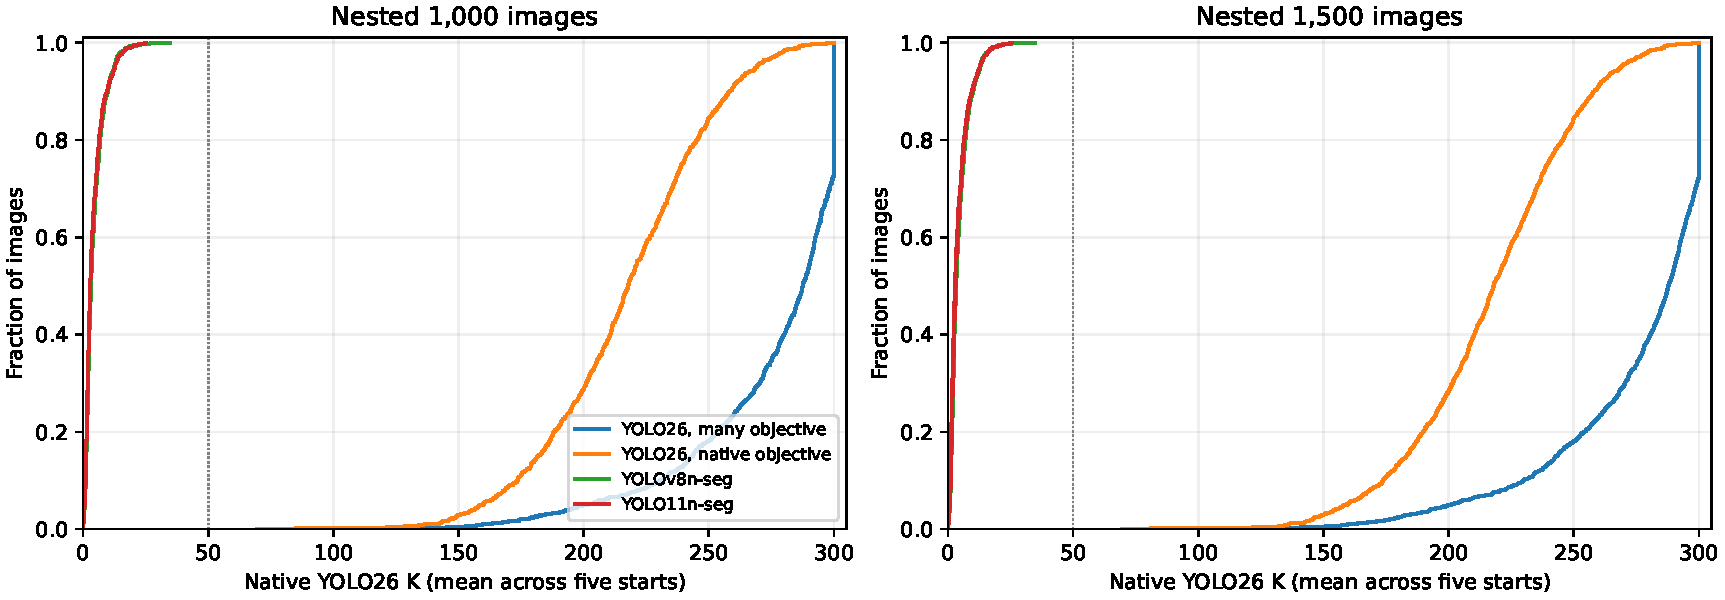
\includegraphics[width=\textwidth]{segmentation_extension/nested1500_native.pdf}\caption{Native YOLO26 count distributions under both transfer sources and both target-specific objectives. Each image contributes its mean count over five starts.}\label{fig:nested1500}\end{figure*}
Every case retains candidate-score vectors, detections, and native outputs. Exact adversarial inputs are retained only for the prospectively selected 64-image audit subset across all objectives and starts; the remaining cases have input hashes and saved-output verification, not full input replay. These count results do not repair the failed timing quality gates and do not establish an end-to-end denial of service.

% Generated from saved CPU summaries by make_laptop.py.
\subsection{Repeated laptop CPU measurement with real attacked inputs}
\label{app:seg-laptop}
After the earlier rejected timing campaigns, a source audit identified a carryover imbalance: duplicate A/A labels had equal absolute positions but unequal preceding clean/attacked workload distributions. The caller also retained the previous output during the next invocation. A new prospective protocol balanced labels jointly by preceding workload and pair position, used the same callable for both labels, and released output after both clocks stopped. These changes form a bundle; the observations do not isolate an allocator, cache or scheduler mechanism. All earlier failures remain rejected.
Two prospectively tagged sessions reuse the same 20 frozen whole-image PGD pairs ($L_\infty=16/255$, 100 steps) and YOLOv8n-seg, with FP32 unfused inference, $640\times640$ native masks, confidence 0.25, IoU 0.45 and a fixed torchvision NMS backend. The i5-1335U laptop worker is pinned to logical CPU 2, one hardware thread of a P-core, with one intra-op and one inter-op thread. AboveNormal priority and HighQoS are process-local; the assistant application tree temporarily avoids CPU 2 and its SMT sibling 3, with journaled restoration. No power-plan or thermal-protection changes are made.
Each image/arm has 48 trials per A/A label; the primary median pools all 96 calls. All trials and spikes are retained. The endpoint spans prepared tensor to native-mask return, excluding output cleanup, decoding, transport, serialization and queueing. Each session independently requires at most two of 22 forward-reference medians outside $\pm3\%$ of baseline, both A/A MDEs at most 1\%, valid load pinning and environment/readback/restoration checks. Intervals below resample the 20 images 20,000 times, RNG seed 20261107; repeats are not independent images.
\begin{table*}[t]\centering
\caption{Two separately gated sessions on the same 20 frozen image pairs. Ratios are geometric means of per-image attack/clean median total latency. Both sessions pass; they are not independent image or device replications.}
\label{tab:seg-laptop}
\begin{tabular}{lrrrr}\toprule
Session & Total ratio [95\% CI] & Clean A/A MDE (\%) & Attacked A/A MDE (\%) & Drift flags\\\midrule
1 & 4.235134 [4.024954, 4.441712] & 0.996622 & 0.213432 & 1/22 \\
2 & 4.222968 [4.007657, 4.433076] & 0.829358 & 0.168182 & 0/22 \\
\bottomrule\end{tabular}\end{table*}
\begin{figure*}[t]\centering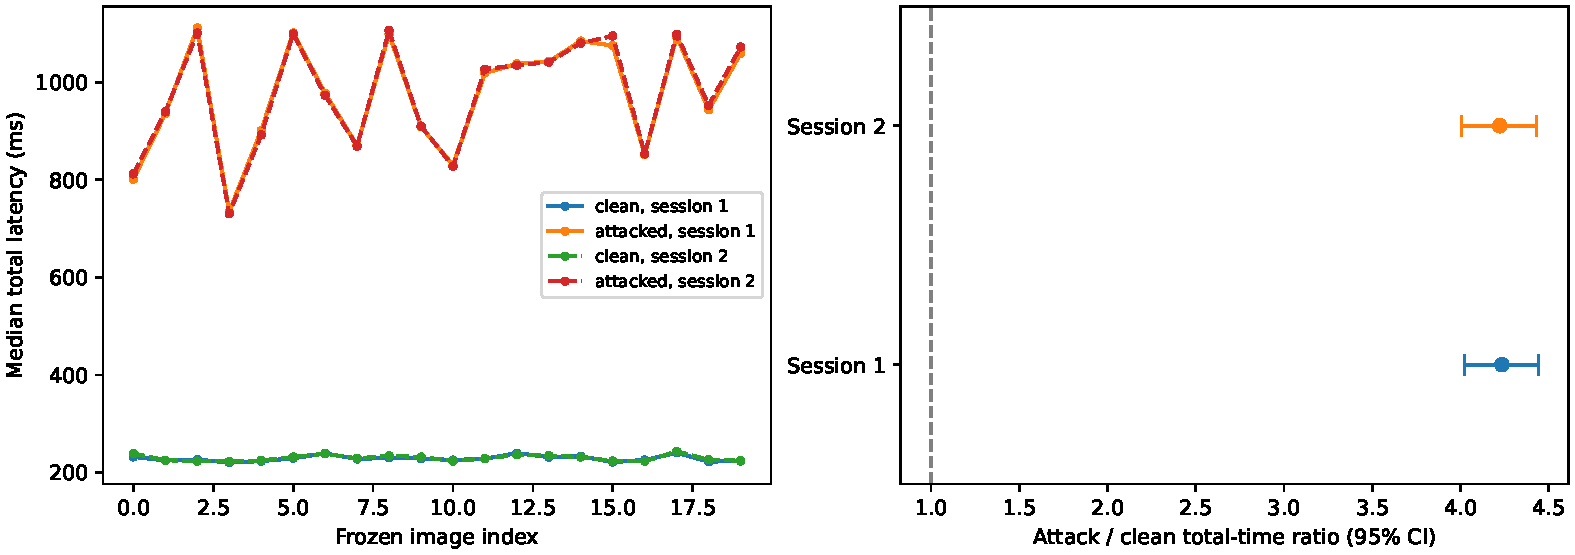
\includegraphics[width=.9\textwidth]{segmentation_extension/laptop_sessions.pdf}\caption{Saved per-image median latency and separate session ratio intervals. The same images and deterministic schedule are shared; no pooled cross-session interval is constructed.}\label{fig:seg-laptop}\end{figure*}
The first session clean MDE is close to the 1\% gate; the unrounded value was used for eligibility. Passing this median-based gate does not establish stable tail latency. Session 1 retains 24/1920 clean and 42/1920 attacked calls exceeding 1.5 times their image-specific median; session 2 retains 14/1920 and 52/1920. Each of these spikes has process-CPU/wall below 0.75. Their cause is unresolved. Process CPU time is coarsely quantized on this Windows installation; PDH nominal frequency is not treated as measured instantaneous clock.
The second session was registered after inspecting the first and reused its configuration without searching additional repeats or cores. Similar estimates are descriptive repeatability evidence, not an equivalence test. Neither session isolates NMS from mask work because isolated-stage profiling was omitted from this corrected total-only schedule. The installed native renderer chunks floating-point interpolation and returns uint8 masks; a monolithic full-float mask allocation is not assumed. Legacy shared hardware-helper line-ending differences between Git and executed working bytes are disclosed in the audit receipt; the prospective lock binds the exact executed SHA.
This result supports increased prepared-tensor computation cost in two sessions on one laptop and one model. It does not establish service denial, deadline misses, camera robustness, universal/localized patch effectiveness, ARM/Pi behavior, or timing validity for the separate 1500-image count cohort. No failed session is pooled into these estimates.

% Generated from saved defense family by make_defense.py.
\subsection{Paired pre-NMS defense timing}
\label{app:seg-laptop-defense}
After the two accepted CPU sessions, a separate prospective protocol fixes two interventions: cap candidates before NMS at 300, or cap retained outputs at 50. Each comparison uses the identical frozen attacked tensor in both arms and a newly measured, interleaved baseline (candidate cap 30000, output cap 300). The device, model, fixed NMS backend, resolution and carryover-balanced duplicate-label schedule follow the laptop method above. Each block has its own smoke and conditional full run, independent quality gate, SHA-bound source/input lock and app-affinity restoration. A temporary probe records the actual compiled-kernel input count outside timing and restores the original function before warmup and measurement.
\begin{table*}[t]\centering
\caption{Predetermined defense comparisons. Only the pre-NMS intervention reached full timing qualification. The failed output-cap smoke is retained and its full run was cancelled, without retry.}
\label{tab:seg-laptop-defense}
\begin{tabular}{lrrrr}\toprule
Intervention & Defended/baseline [95\% CI] & Baseline A/A MDE (\%) & Defended A/A MDE (\%) & Drift flags\\\midrule
Pre-NMS cap 300 & 0.526773 [0.507007, 0.548921] & 0.149061 & 0.314700 & 1/22 \\
Output cap 50 & Not qualified; full cancelled & --- & --- & 1/4 (smoke) \\
\bottomrule\end{tabular}\end{table*}
For the pre-NMS cap, total latency decreases by 47.322709\% [pointwise 95\% CI 45.107882, 49.299341]. The mean paired difference of image medians is -468.920147 ms [95\% CI -510.113507, -425.613187]. Each interval uses the registered 20000 image-bootstrap replicates; these intervals are not simultaneous family-wise intervals.
All 20 image log ratios have the same negative sign. The two-sided exact sign-flip calculation enumerates all $2^{20}$ assignments, giving $p=2/2^{20}$; Holm adjustment over the two registered comparisons gives $p_{\mathrm{Holm}}=4/2^{20}$. The unmeasured/failed output-cap comparison contributes a testing placeholder of one to preserve family size; that value is not a finding of no effect. Sign-flip inference assumes sign exchangeability under the null and does not create random-population sampling or additional image independence.
Observed kernel inputs fall from 1726--3744 to exactly 300 for every image. Retained masks change from a median of 270.5 (range 177--300) to 98 (84--118). Thus the intervention bounds kernel input but retains nonzero mask work; this total-pipeline contrast does not separately attribute savings to NMS and mask rendering. All raw spikes remain, including 50/1920 baseline and 29/1920 defended calls exceeding 1.5 times their image-specific median, each with process-CPU/wall below 0.75.
\begin{figure*}[t]\centering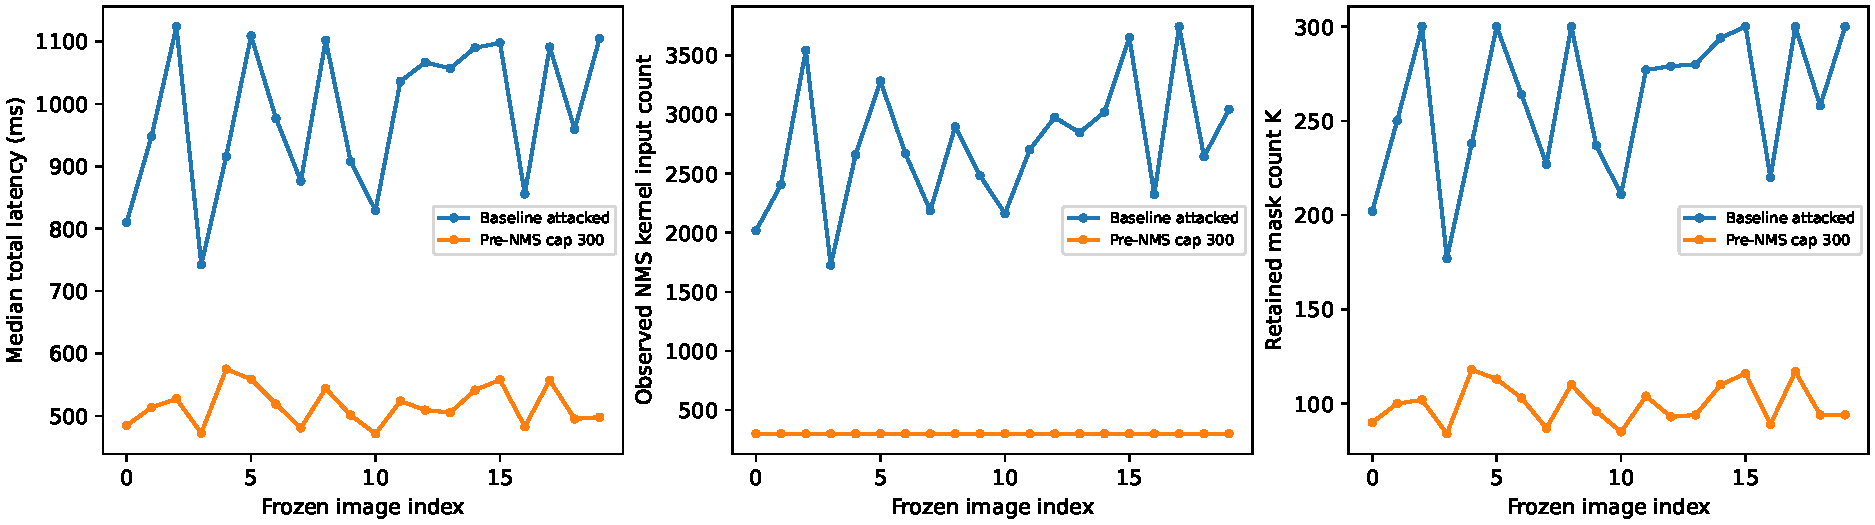
\includegraphics[width=.98\textwidth]{segmentation_extension/laptop_defense.pdf}\caption{Qualified pre-NMS intervention: per-image median total latency, observed compiled-NMS input count, and retained mask count. Counts and timing have separate axes and units.}\label{fig:seg-laptop-defense}\end{figure*}
The output-cap smoke had a forward-reference ratio of 1.0376245029873103 at its first image, exceeding the registered 3\% bound; its apparently lower timings remain diagnostic and are not used as a qualified defense estimate. Both blocks restored all 45 application processes. The study tests fixed saved perturbations, not an adaptive adversary trained against the cap. The earlier clean-accuracy evaluation used confidence 0.001 and letterboxing, unlike this confidence-0.25 square-tensor latency protocol; no jointly matched accuracy--latency curve or availability guarantee is inferred.

% Generated from the closed, failed component campaign by make_components.py.
\subsection{Prepared-input component controls: qualification failures}
\label{app:seg-laptop-components}
Following the accepted total-pipeline sessions, a separate prospective protocol fixes two prepared-input endpoints on the same laptop and frozen image pairs: blocks of 64 original torchvision NMS calls on captured boxes/scores, and one native mask-renderer call on cached prototypes and retained detections. NMS per-call estimates divide whole-block timing by 64 and include the Python facade/loop/index release; mask output release occurs after timing. Preparation is outside timing. These different cache and lifetime scopes are not an additive decomposition of the earlier pipeline.
The NMS two-image smoke completes 384 trials with zero of four reference blocks flagged, permitting one 20-image full run. The full run completes all 3840 trials and all input-immutability, prediction/count, affinity and source audits, but fails its registered reference-drift criterion: 20 of 22 blocks are flagged (maximum allowed: two). Nineteen flagged references are faster than the initial reference and one is slower. Therefore this failure cannot be described simply as progressive slowing; the physical cause is unresolved.
The full NMS duplicate-label A/A MDEs are 0.340730\% (clean) and 0.095851\% (attacked). Passing these two precision bounds does not override the failed reference gate.
The distinct, predetermined native-mask smoke completes 384 trials but flags its final reference (ratio 1.0328367896175703), exceeding the smoke allowance of zero flags. Its full run is cancelled. No component is repeated, no gate is relaxed, and neither contrast is eligible for primary inference. Testing placeholders of one preserve the declared two-comparison family but are not evidence of no effect. Apparent component ratios remain in diagnostic artifacts only.
\begin{figure*}[t]\centering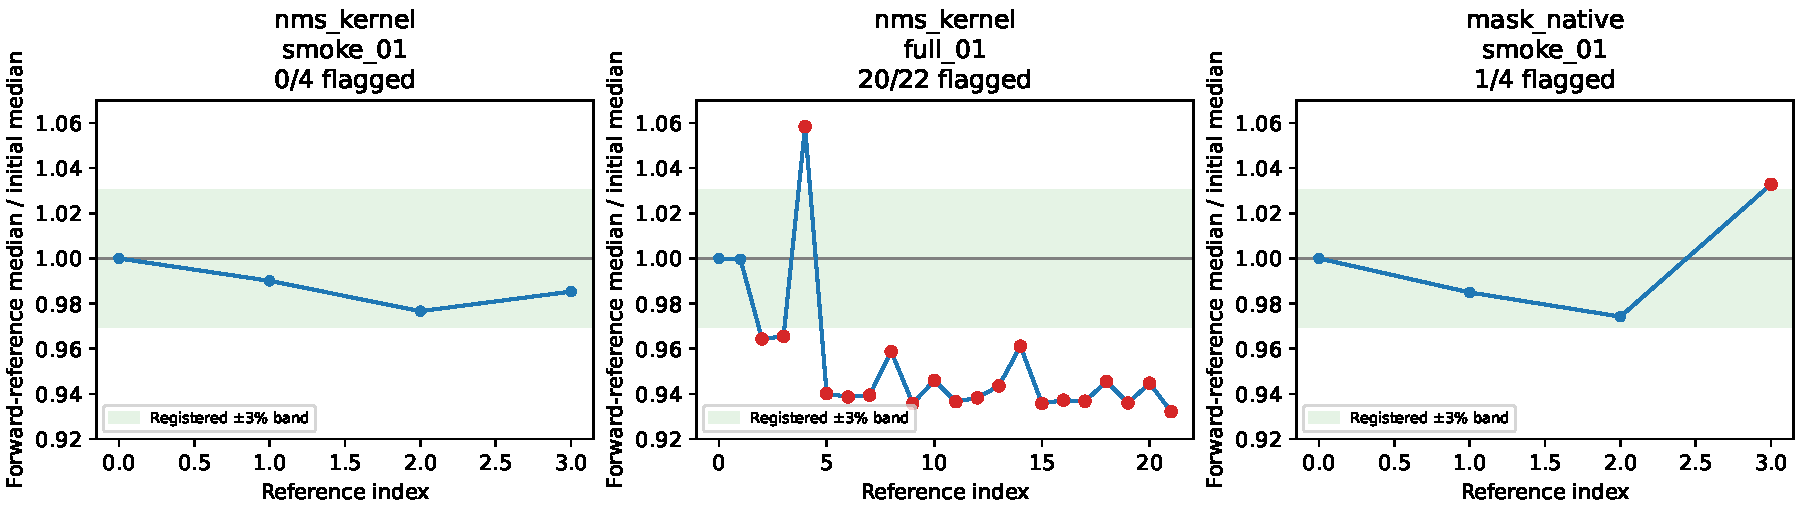
\includegraphics[width=.98\textwidth]{segmentation_extension/laptop_components.pdf}\caption{All reference blocks in the closed component campaign. Shading marks the registered 3\% band; red points are flagged. Both full component contrasts remain unqualified.}\label{fig:seg-laptop-components}\end{figure*}
All three completed runs restore the original affinity of 45 application processes. Failed component controls do not invalidate separately qualified total-pipeline or paired-defense sessions, and do not supply additional evidence of service denial, tail stability, physical attacks or ARM performance.

% Generated from saved forward-only traces by make_reference_trace.py.
\subsection{Forward-reference diagnostic without NMS or masks}
\label{app:seg-forward-reference}
A subsequent prospective diagnostic records the forward-reference workload alone on the same CPU, model and one fixed clean image. Two fresh processes each execute 12 blocks of three fixed warmup forwards and 15 timed forwards: one continuous cadence and one with a two-second pause between blocks. The registered order is continuous first. PDH is recorded after every timed forward, and each output is released after both clocks. All 360 samples complete, pin-load checks pass, and all 45 application affinities are restored before analysis.
The continuous trace flags 4/12 block medians and the paused trace flags 2/12 against their own first-block median using the descriptive 3\% threshold; every flagged block is faster. Thus reference drift exceeding this threshold is observed even without NMS or mask work. This does not uniquely identify the mechanism of the earlier component failures. There is one process per cadence and the fixed order confounds cadence with session/time; the flag counts are not evidence that pausing improves stability. No CI, p-value, A/A MDE or attack qualification is inferred, no baseline is replaced, and the finite protocol stops without retry.
\begin{figure*}[t]\centering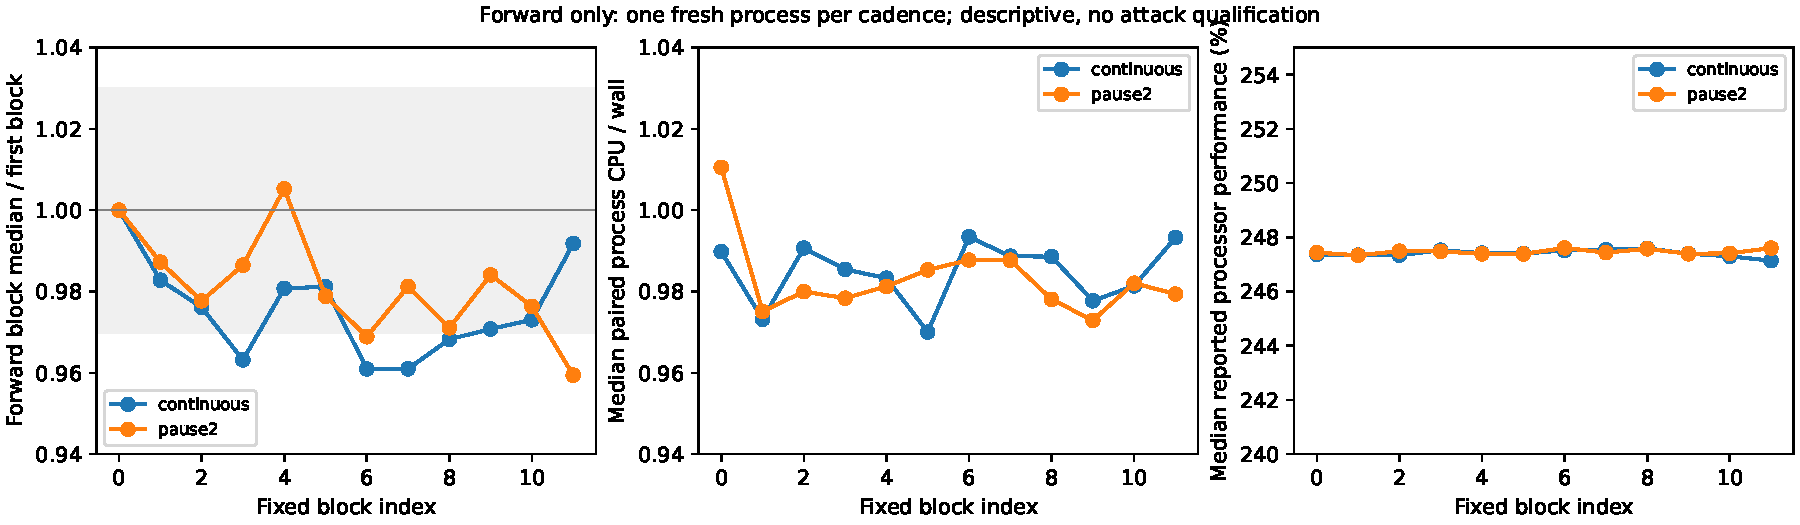
\includegraphics[width=.98\textwidth]{segmentation_extension/laptop_reference_trace.pdf}\caption{Forward-only diagnostic: block wall-median ratios, median paired process-CPU/wall values, and median reported processor-performance counter. Shading marks the descriptive 3\% band. Interval counters and quantized process CPU do not identify thermal, clock, cache or scheduling causes.}\label{fig:seg-forward-reference}\end{figure*}
The initial runtime, pin-load and cache context differs from the component workload. These controls retain all observations, supply no ARM or service-denial result, and do not promote either previously failed component contrast.

% Generated from the closed P2 smoke by make_pcores.py.
\subsection{Two physical P cores: smoke rejected}
\label{app:seg-laptop-pcores}
A separate prospective protocol fixes logical CPUs [0,2], one thread from each physical P core, with two intra-op and one inter-op threads. The same corrected whole-pipeline worker, fixed NMS backend, model and saved input pairs are reused. The owned application temporarily excludes both P cores and their SMT siblings [0,1,2,3]. This changes the application placement relative to the historical one-core sessions, so cross-profile speedup is not an identified treatment effect.
The single two-image smoke completes all 384 timing trials and passes both pin-load checks (approximately 1.95 effective cores). All 45 application affinities are restored. However, two of four forward references are flagged: ratios 1.0953159727928494 before the first image and 1.0317927329528502 at the end. The registered smoke allows no flags, so the full 20-image run is cancelled without retry, additional cores or a warmup sweep. Apparent latency ratios and the two-image A/A estimates remain diagnostic only; no qualified multi-core attack estimate follows.
All four clean/attacked prediction hashes differ from the historical one-core outputs, while the candidate and retained-mask counts are unchanged for these two images. These numerical observations are retained rather than treated as an image-exclusion rule. Process-CPU/wall values on two cores represent effective CPU use and may exceed one; the PDH query covers CPU0 only. This rejected smoke does not establish that multi-core pinning is impossible, identify a thermal or scheduling cause, or support a service-denial conclusion.
\begin{figure*}[t]\centering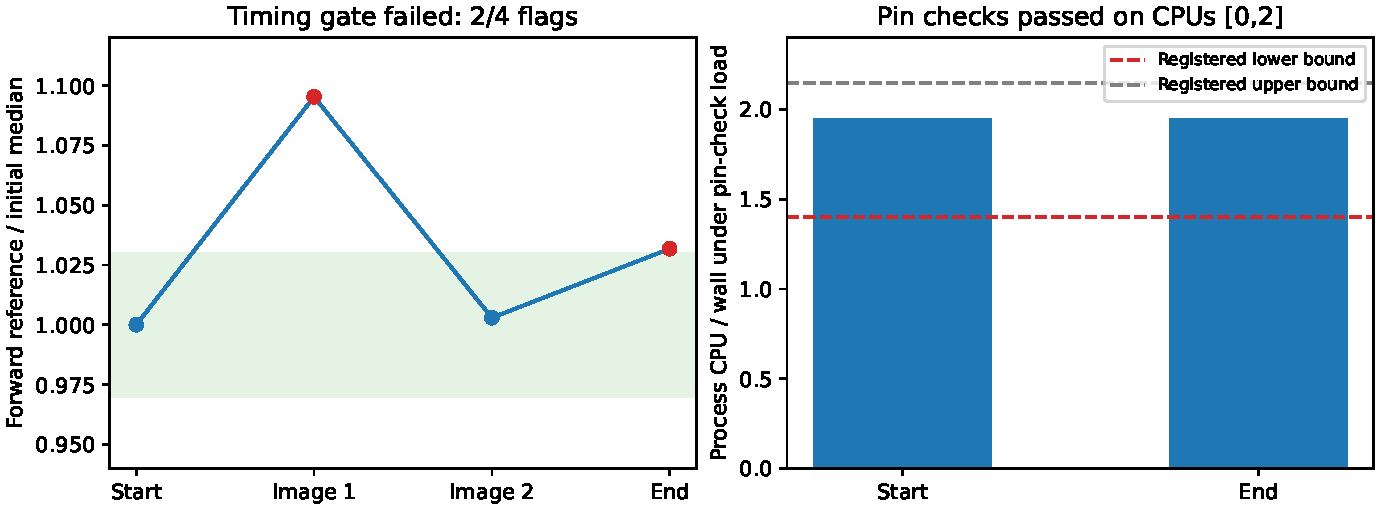
\includegraphics[width=.90\textwidth]{segmentation_extension/laptop_pcores.pdf}\caption{Two-P-core smoke: reference-timing failure alongside passing start/end pin-load checks. These are distinct gates; passing affinity verification does not override timing instability.}\label{fig:seg-laptop-pcores}\end{figure*}

